\documentclass[11pt]{exam} 
\usepackage{tkz-euclide}
\begin{document} 
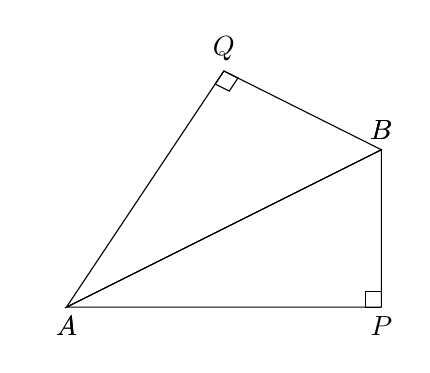
\begin{tikzpicture} 
        \coordinate (P) at (4, 0) {};
        \coordinate (A) at (0, 0) {};
        \coordinate (B) at (4, 2) {};
        \coordinate (Q) at (2, 3) {};
        \draw (Q)node[above]{$Q$}--(A)node[below]{$A$}--(B)node[above]{$B$}--cycle;
        \draw (B)node[above]{$B$}--(A)node[below]{$A$}--(P)node[below]{$P$}--cycle;
\tkzMarkRightAngle[size=.2](B,P,A);
\tkzLabelAngle[dist=.5](P,A,B){};
\tkzMarkRightAngle[size=.2](B,Q,A);
\tkzLabelAngle[dist=.5](Q,A,B){};
\end{tikzpicture}
\end{document}